\section{Openflow background}
\label{section:inflex:background}

A valuable development in assisting traffic management has been the emergence of \ac{SDN}, which can facilitate vastly improved flexibility for scalable, policy-based network control.
Software defined networks decouple the data plane and control plane, allowing both to evolve independently.
A traditional instantiation of a software defined network for data centres is shown in figure \ref{fig:ofparch}.
Each physical host runs a number of virtual machines, each connected locally through a edge, software-based switch (such as OpenVSwitch \cite{openvswitch}) running on the underlying physical host operating system, which will be denoted as \emph{dom0}.
This switch is in turn connected to further forwarding devices, ensuring access to a wider network.
The forwarding logic of each device can be accessed and configured by a controller through the establishment of a control channel through a common protocol, of which Openflow is the most widely used \cite{McKeown:2008:OEI:1355734.1355746}.
Both software and physical switches are indistinguishable from a controller's perspective: \emph{how} a device implements Openflow is immaterial, so long as a forwarding device conforms to the given \ac{API}.

\begin{figure}
    \centering
    \begin{subfigure}[b]{0.5\linewidth}
    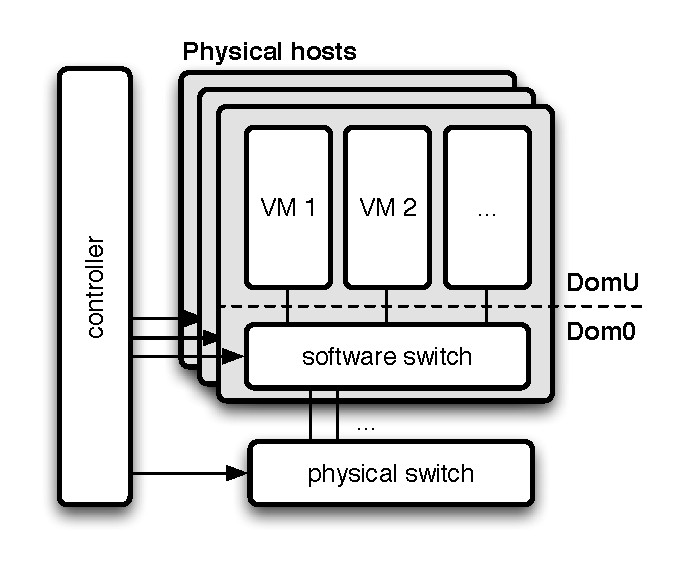
\includegraphics[width=0.9\linewidth]{figures/inflex/ofparch}
    \caption{\label{fig:ofparch}}
    \end{subfigure}%
    \begin{subfigure}[b]{0.5\linewidth}
    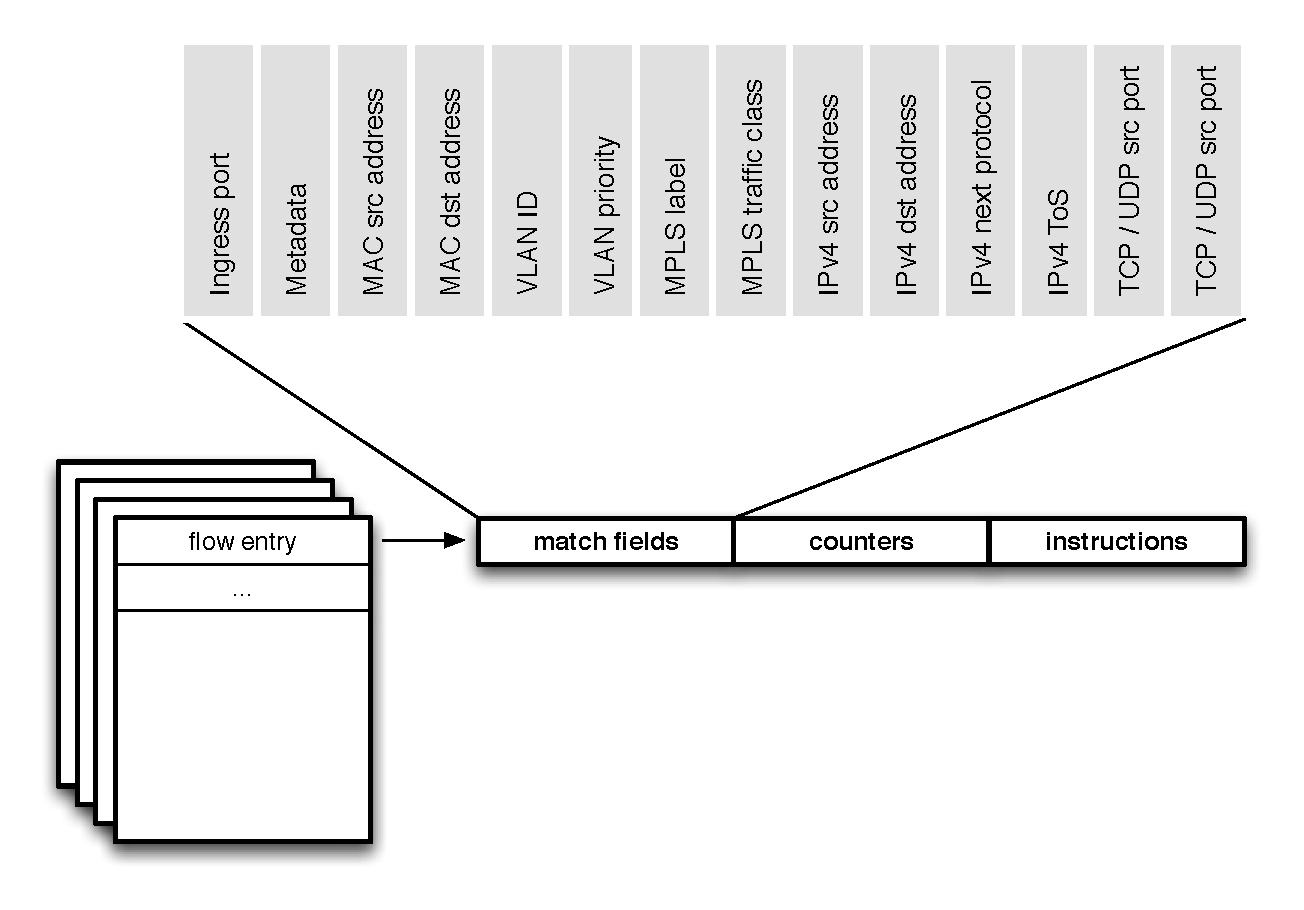
\includegraphics[width=0.9\linewidth]{figures/inflex/ofptable}
    \caption{\label{fig:ofptable}}
    \end{subfigure}
    \caption{Openflow (\subref{fig:ofparch}) architecture and (\subref{fig:ofptable}) flow entry structure.}
\end{figure}

% flow table / entry
An Openflow flow table is composed of multiple flow entries, shown in figure \ref{fig:ofptable}.
Each flow entry is comprised of a pattern to be matched, and the corresponding \emph{instructions} to be executed. 
The \emph{match fields} over which an entry can be compared span from data link to transport layers, covering not only source and destination addresses at each protocol header, but also traffic classes and labels for \ac{VLAN}, \ac{MPLS} and \ac{IPv4} headers.
% instructions?
Additionally, a \emph{counter} keeps track of the number of times the entry is matched.
If more than one matching entry is found, only the entry with the highest \emph{priority} is processed.
Finally, each entry has a pair of associated \emph{timeout} values: a soft timeout, within which an entry is expired if no matching packet arrives, and a hard timeout, by which an entry is irrevocably expired.
If neither timeout is set, a flow entry persists indefinitely.

% processing pipeline
An Openflow switch in turn maintains multiple flow tables.
Every packet received at an Openflow compliant switch is processed along a pipeline which starts by matching the packet against \emph{table 0}.
From this first, default table, corresponding \emph{instructions} may redirect the packet for further matching against another table, thereby chaining processing.
This pipeline processing ceases once a matching entry fails to include a redirection request, with the accumulated instruction set being executed.
In addition to redirections, valid instructions include modifying packet fields, pushing and popping packet tags, and defining through which ports a packet should be forwarded.
%instructions?
If at any point no matching entry is found, the packet is buffered at the switch, and the truncated packet header is sent to the controller.
% controller
Based on the header contents, a controller may decide to install a new flow entry on the switch, or allow the packet to be dropped altogether.
Compared to the underlying abstracted network elements which compose the data path, the controller is often expected to be entirely software based, and as such is not constrained in how it should process packets.
In practice, this freedom is curbed as increasing complexity at the controller both reduces the rate at which packets are processed, as well as increasing latency for packets buffered at the switch.

% 2 tradeoffs: 
\ac{SDN} provides an abstraction over which different architectural paradigms can be adapted and even coexist.
It does not however prescribe or advocate a specific design -- network practitioners must still consider system properties when grappling with fundamental trade-offs affecting consistency, isolation, reliability and efficiency.
Some of the design considerations for scalable traffic management were previously described in section \ref{section:inflex:design}.
The overall performance of the described architecture is subject to two further critical trade-offs.
% - granularity vs speed
Firstly, the granularity at which flow entries are installed determines how often a controller is called to intervene.
While installing an entry at a flow granularity may allow fine-grained control of resources, it increases both the load on the controller and the latency of the withheld packet.
Conversely, as the granularity becomes coarser, the overhead incurred by the controller is reduced at the cost of flexibility in controlling traffic.
% - omniscience vs fault tolerance
Secondly, controller placement is critical \cite{Heller:2012:CPP:2342441.2342444}.
At one extreme, a fully centralized controller is omniscient within a domain at the expense of reliability and scalability.
At the other, a distributed system of controllers forsakes consistency and liveness in order to scale robustly.
